\documentclass[pdf,unicode]{beamer}
\usepackage[T2A]{fontenc}       %поддержка кириллицы
\usepackage[utf8]{inputenc}   %пока бибтех не дружит до конца с юникодом
\usepackage[russian]{babel}     %определение языков в документе
\usepackage{amssymb,amsmath}    %математика
\usepackage{graphicx}
\usepackage{color}
\usepackage{bm}
\usepackage{epsfig,float}
\usepackage[format=plain,labelsep=period,justification=centerlast]{caption}  %оформление подписей к рисункам

\def\Year{\expandafter\YEAR\the\year}
\def\YEAR#1#2#3#4{#3#4}

\setbeamertemplate{caption}[numbered]
\renewcommand{\tiny}{\fontsize{5}{8.4pt}\selectfont}
% Тема презентации
%\usetheme[nonav, numbers, totalnumbers, minimal, nologo]{Statmod}
%\usetheme{Dresden}
%\usetheme{Goettingen}
\usetheme{Warsaw}
%%%%%%%%%%%%%%%%%%%
%% Выбор шрифтов %%
\usefonttheme[onlylarge]{structurebold}

% Привычный шрифт для математических формул
\usefonttheme[onlymath]{serif}

% Более крупный шрифт для подзаголовков титульного листа
\setbeamerfont{institute}{size=\normalsize}
%%%%%%%%%%%%%%%%%%%

% Если используется последовательное появление пунктов списков на
% слайде (не злоупотребляйте в слайдах для защиты дипломной работы),
% чтобы еще непоявившиеся пункты были все-таки немножко видны.
\setbeamercovered{transparent} \setlength\abovecaptionskip{-10pt}
\setlength\belowcaptionskip{-10pt}


%%%%%%%%%%%%%%%%%%
%%% Сокращения %%%
% Синий цвет выделения
\setbeamercolor{color1}{bg=blue!60!black,fg=white}

%%%%%%%%%%%%%%%%%%
%\input{monogr}
%\input{mondef}
%\input{monscrt}
\title[Ультратонкие магнитные пленки]{Ультратонкие магнитные пленки}
\subtitle{\textbf{Особенности моделирования и структур}}
\author[Ватолкин М.А.]{\rule{0pt}{1cm} автор: {Ватолкин Михаил Александрович}}
\institute{кафедра теоретической физики ОмГУ}
\date{Омск -- 20\Year}

\begin{document}

\begin{frame}
  % создаём титульный лист
  \maketitle
\end{frame}
%%%%%%%%%%%%%%%%%%%%%%%%%%%%%%%%%%%%%%%%%%%%%%%%%%%%%%%%%%%%%%%%%%

\begin{frame}
\frametitle{Введение}
Исследование пленок позволяет получать новую и ценную информацию о магнитных свойствах и явлениях ферромагнетиков.\\ 
Одно из таких явлений - гигантское магнитосопротивление.\\
Также очень важно, что в пленках можно реализовать структурные состояния, которые трудно или невозможно получать в обычных (массивных или обьемных) магнитных образцах.

\end{frame}
%%%%%%%%%%%%%%%%%%%%%%%%%%%%%%%%%%%%%%%%%%%%%%%%%%%%%%%%%%%%%%%%%%

\begin{frame}
\frametitle{Особенности  медленной динамики}
	По сравнению с объемными магнитными системами, в которых медленная
	динамика и эффекты старения проявляются вблизи критической точки, магнитные сверхструктуры с
	наномасштабной периодичностью дают возможность
	увеличить время релаксации за счет эффектов, связанных с увеличенной в этих структурах характеристической корреляционной длиной спин-спиновых
	корреляций.По этой причине эффекты старения и
	неэргодичности могут наблюдаться в мультислойных
	магнитных структурах в более широком температурном интервале по сравнению с объемными магнитными системами
\end{frame}
%%%%%%%%%%%%%%%%%%%%%%%%%%%%%%%%%%%%%%%%%%%%%%%%%%%%%%%%%%%%%%%%%%

\begin{frame}
    \frametitle{Временные корреляции}
    Для спиновой системы, характеризуемой спиновой плотностью $S(x,t)$, временная корреляционная функция определяется выражением



$ C(t,t_w)=$   ${1\over{V}}\int<S(x,t)S(x,t_w)>d^d x$  \\
 ~~~~~~~~~~~~~ $-{1\over{V}} \int<S(x,t)><S(x,t_w)>d^d x$\\

где $t$ - время наблюдения, $t_w$ - время ожидания, \\$d$ - размерность пространства, $x$ -$d$-мерный радиус-вектор.
\end{frame}
%%%%%%%%%%%%%%%%%%%%%%%%%%%%%%%%%%%%%%%%%%%%%%%%%%%%%%%%%%%%%%%%%%

\begin{frame}
    \frametitle{Временные корреляции}

  \begin{figure}
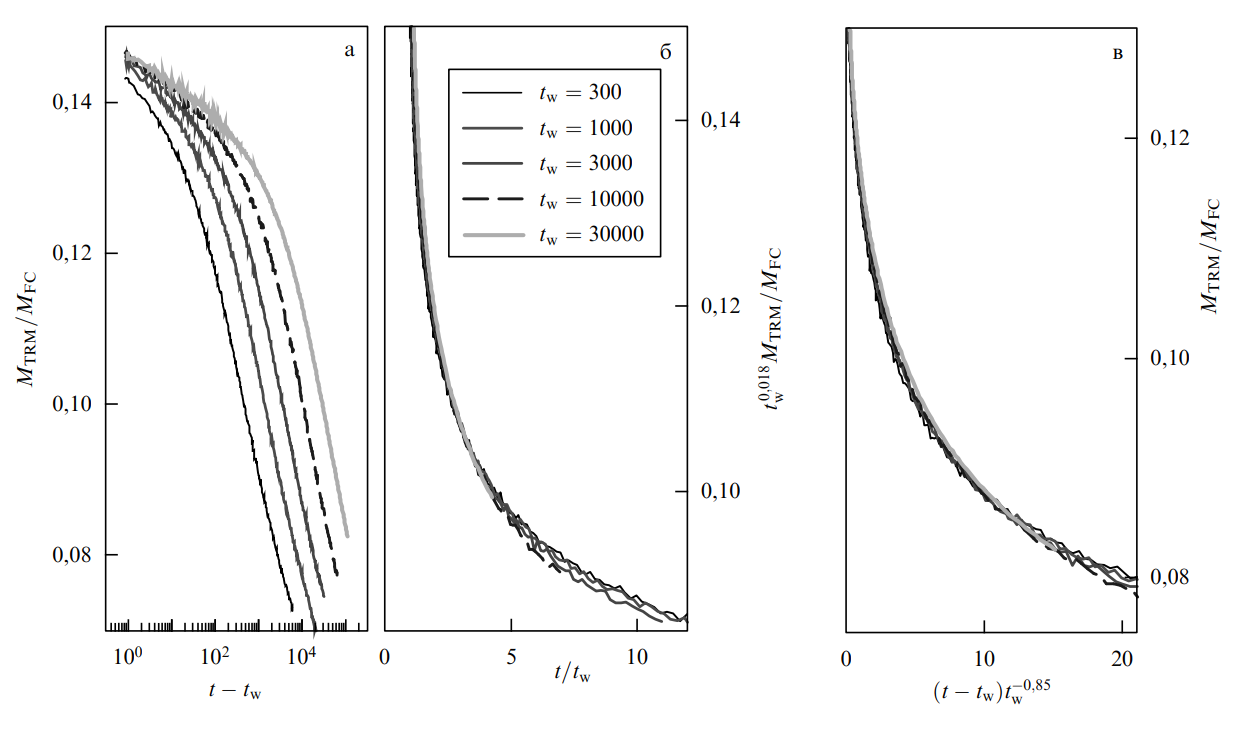
\includegraphics[width=1\textwidth]{Image1.png}
	\caption{\scriptsize Эффекты старения(а) и результаты проверки скейлинговых форм: канонического старения(Б) и субстарения(В), выявленные в зависимости термостатичной намагниченности $M_{TRM}$ от времени наблюдения $t - t_w$ и времени ожидания $t_w$, при эволюции из высокотемпературного начального состояния}

\end{figure}
\end{frame}
\begin{frame}

\frametitle{Функция отклика}
Функция отклика на малое внешнее магнитное поле $h(x,t_w)$ прикладываемое к системе в момент $t_w$ задается соотношением:
\begin{equation*}
R(t,t_w) = \frac{1}{V} {\int d^d x \frac{\delta \langle S(x,t)\rangle}{\delta h(x,t_w)} }\bigg|_2
\end{equation*}
где $t$ - время наблюдения, $t_w$ - время ожидания, \\$d$ - размерность пространства, $x$ -$d$-мерный радиус-вектор.
\end{frame}
%%%%%%%%%%%%%%%%%%%%%%%%%%%%%%%%%%%%%%%%%%%%%%%%%%%%%%%%%%%%%%%%%%



%%%%%%%%%%%%%%%%%%%%%%%%%%%%%%%%%%%%%%%%%%%%%%%%%%%%%%%%%%%%%%%%%%

%%%%%%%%%%%%%%%%%%%%%%%%%%%%%%%%%%%%%%%%%%%%%%%%%%%%%%%%%%%%%%%%%%
\begin{frame}
\frametitle{Флуктуационно-диссипативная теорема}
Стоит уточнить, что функция отклика $R(t,t_w)$ не может быть непосредственно измерена экспериментально или получена методами компьютерного моделирования. Поэтому более удобной величиной является интегральная характеристика -- динамическая восприимчивость $(\chi)$, которая может быть рассчитана методами Монте-Карло на основе следующего соотношения:
\begin{equation}
\chi(t,t_w) = \frac{1}{L^2h^2} \sum\limits_i \overline{\langle h_i(t_w)S_i(t)\rangle},
\end{equation}
где $h_i$-малое случайное магнитное поле, черта сверху обозначает процедуру усреднения
по различным реализациям магнитного поля на узлах решетки.
\end{frame}
%%%%%%%%%%%%%%%%%%%%%%%%%%%%%%%%%%%%%%%%%%%%%%%%%%%%%%%%%%%%%%%%%%
\begin{frame}

\frametitle{Особенности поведения намагниченности}
Для более точного определения критических температур рассматривались системы с различными линейными размерами $L = 16,24,32,64$ рассчитывались такие характеристики как "шахматная" намагниченность	\\
$M_stg = m_1 - m_2$, где $m1$ и $m2$ - намагниченность пленок\\ и шахматная теплоемкость \\$C_h = [<E^2>-<E>^2]/(k_b T)^2 N_s$, где $N_s$ - число спинов в пленке.
\end{frame}
\begin{frame}

\frametitle{Особенности поведения намагниченности}

\begin{figure}
	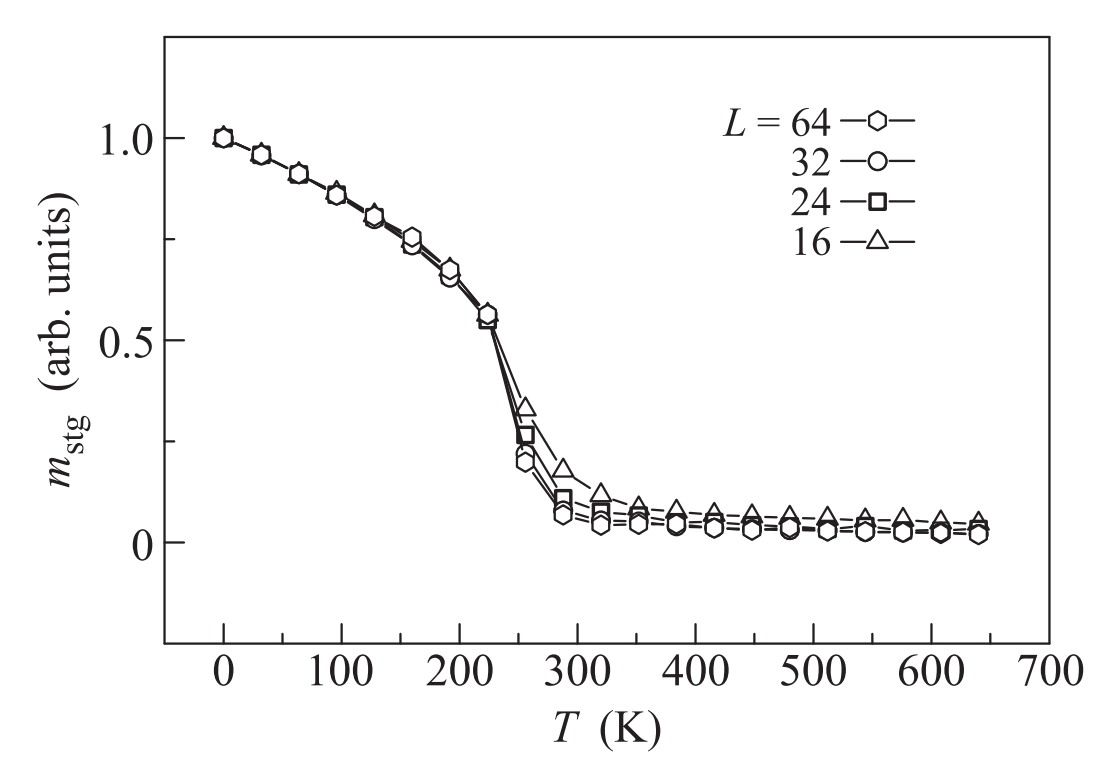
\includegraphics[width=1\textwidth]{Image2.png}
	\caption{\scriptsize Температурное поведение "шахматной" намагниченности $M_stg(T,L)$}
	
\end{figure}
\end{frame}
\begin{frame}
\frametitle{Особенности поведения теплоемкости}

\begin{figure}
	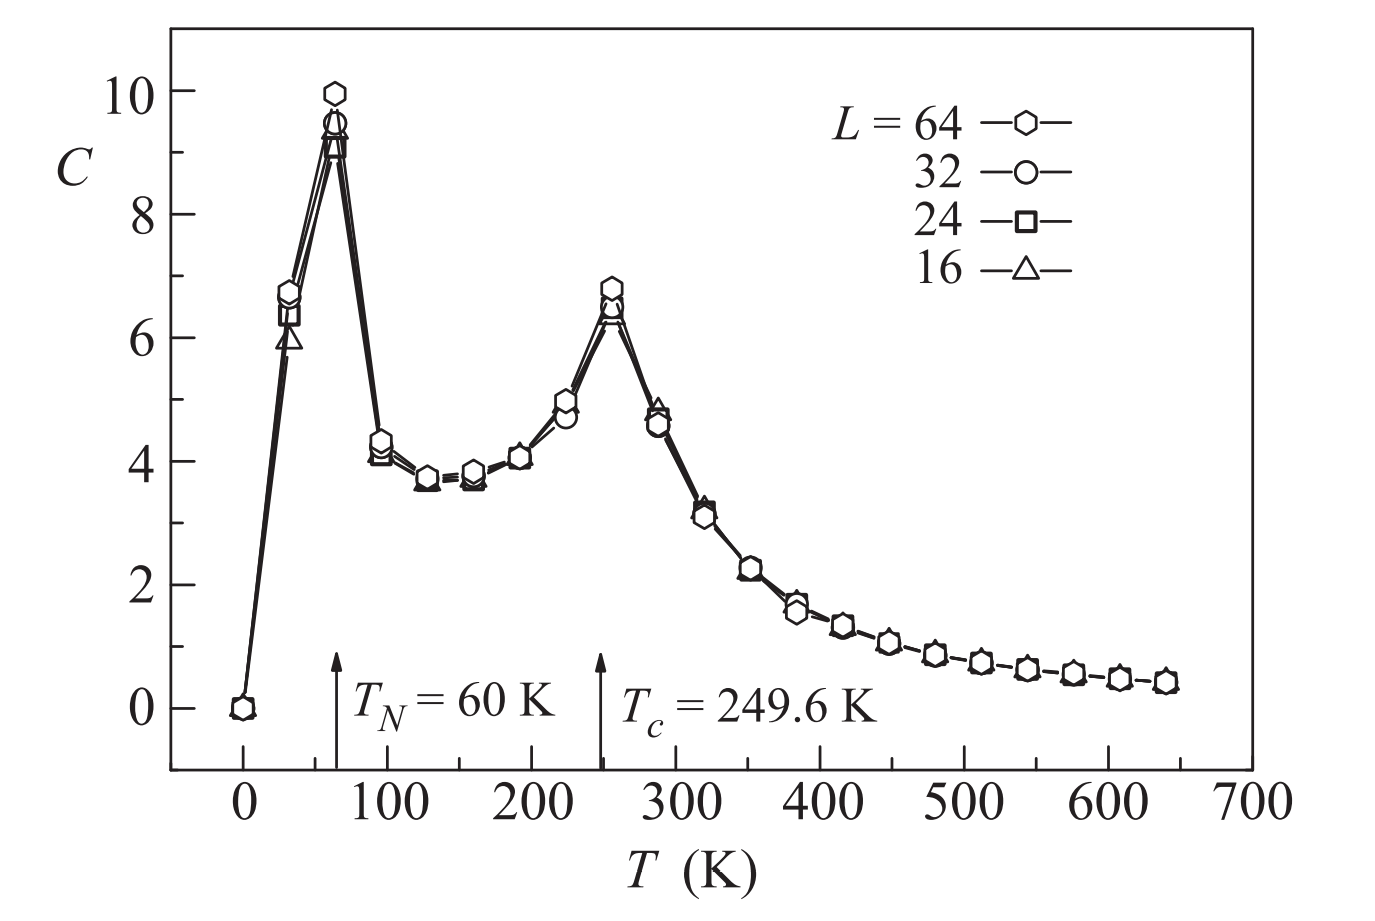
\includegraphics[width=0.8\textwidth]{Image3.png}
	\vspace{5pt}
	\caption{\scriptsize  Температурное поведение теплоемкости \\~~~~$C_h = [<E^2>-<E>^2]/(k_b T)^2 N_s$}
	
\end{figure}
\end{frame}

\begin{frame}
\frametitle{Заключение}
Полученные результаты могут найти свое применение в экспериментальном исследовании неравновесных свойств критической динамики различных структур. Кроме того, они должны учитываться при создании приборов на основе мультислойных магнитных пленок.
\end{frame}




\end{document}
